\begin{frame}
    \frametitle{Aplicación: Siguiendo una trayectoria}
    \note{Información extraída de https://youtu.be/pEVsedl2KO4?si=_cwQpRPPUnQ04B3c}
    
    \begin{center}
        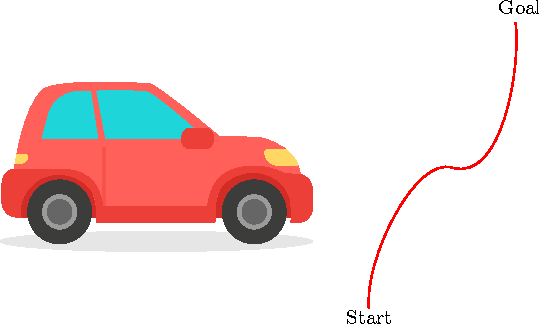
\includegraphics[width=0.6\columnwidth]{images/tracking_trajectory.pdf}
    \end{center}
    
\end{frame}

\begin{frame}
    \frametitle{Arquitectura de control}
    \note{Información extraída de https://youtu.be/pEVsedl2KO4?si=_cwQpRPPUnQ04B3c}
    
    \begin{center}
        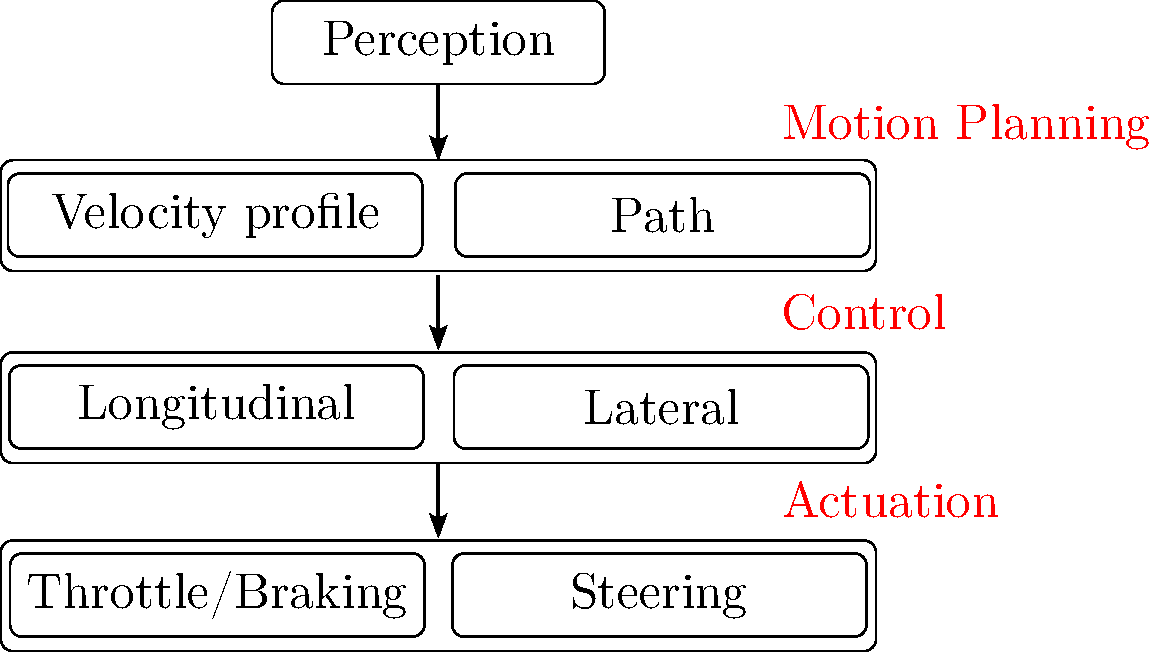
\includegraphics[width=0.8\columnwidth]{images/control_architecture2.pdf}
    \end{center}
    
    \note{Percepción: a través de los sensores armar un mapa del entorno}
    \note{Trayectoria = camino +perfil de velocidades. En cada pose del camino debemos saber con qué velocidad tenemos que llegar. Que cada punto de la trayectoria tenga un perfil de velocidad permite que el robot pueda moverse de manera suave de una pose a la otra.}
    \note{El control se divide en dos partes: longitudinal y lateral. El control Longitudinal hace referencia sobre la dirección de movimiento, es decir controlar la velocidad lineal. El control Lateral hace referencia que el robot este cerca del camino a seguir.}
\end{frame}

\begin{frame}
    \frametitle{Generación de trayectorias}
    \note{Información extraída de https://youtu.be/pEVsedl2KO4?si=_cwQpRPPUnQ04B3c}
    
    \begin{center}
        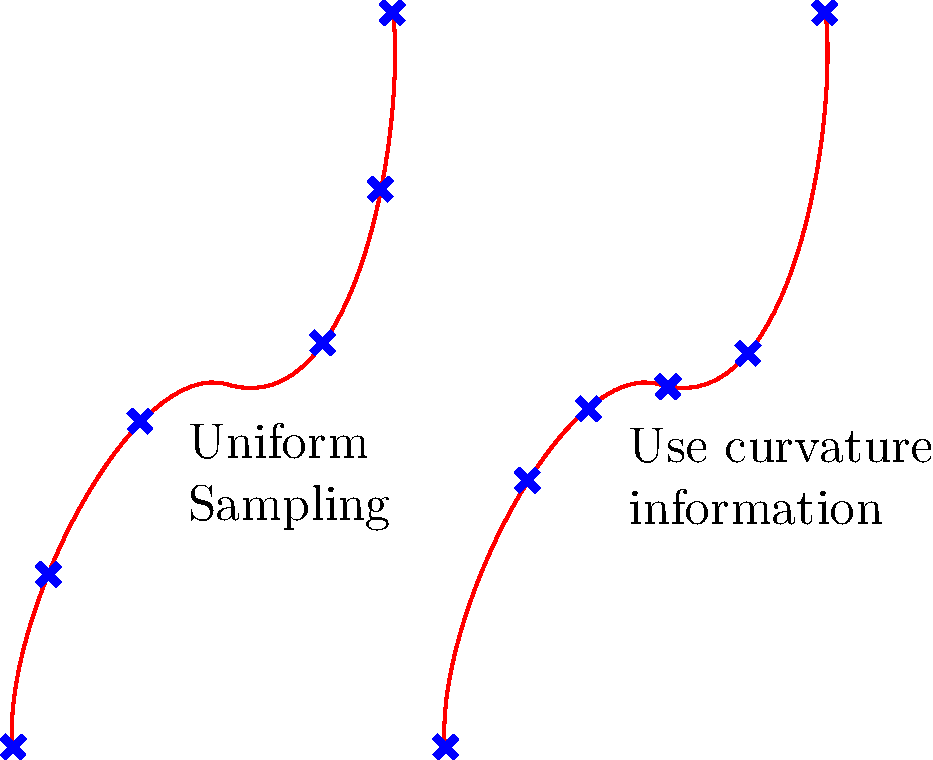
\includegraphics[width=0.6\columnwidth]{images/trajectory_generation.pdf}
    \end{center}
    
\end{frame}

\begin{frame}
    \frametitle{Ackermann Steering}
    \note{Información extraída de https://youtu.be/pEVsedl2KO4?si=_cwQpRPPUnQ04B3c}
    
    \begin{center}
        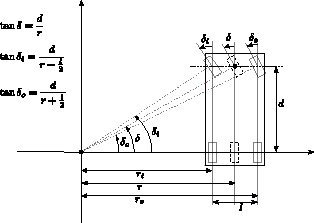
\includegraphics[width=0.6\columnwidth]{images/ackermann_steering.pdf}
    \end{center}
    
\end{frame}

\begin{frame}
    \frametitle{Ackermann Kinematics}
    \note{Información extraída de https://youtu.be/pEVsedl2KO4?si=_cwQpRPPUnQ04B3c}
    
    Estado: $\begin{bmatrix} x & y & \theta & \delta \end{bmatrix}^{\top}$ con $\delta = \tan^{-1}{\left(\frac{d}{r}\right)}$
    
    Control: $\begin{bmatrix} v & \dot{\delta} \end{bmatrix}^{\top}$
    
    
    \begin{center}
        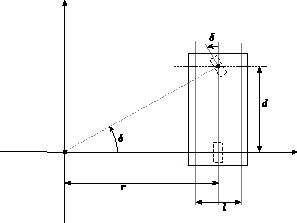
\includegraphics[width=0.6\columnwidth]{images/ackermann_kinematics.pdf}
    \end{center}
    
\end{frame}

\begin{frame}
    \frametitle{Control}
    \note{Información extraída de https://youtu.be/pEVsedl2KO4?si=_cwQpRPPUnQ04B3c}
    
    Restricciones:
    
    $v < v_{\max}$
    
    $\delta < |\delta_{\max}|$
    
    
    \begin{center}
        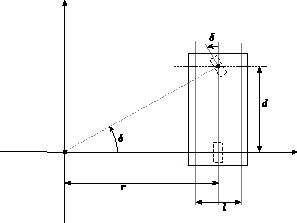
\includegraphics[width=0.6\columnwidth]{images/ackermann_kinematics.pdf}
    \end{center}
    
\end{frame}

\begin{frame}
    \frametitle{Longitudinal Control}
    \note{Información extraída de https://youtu.be/pEVsedl2KO4?si=_cwQpRPPUnQ04B3c}
    
    \begin{center}
        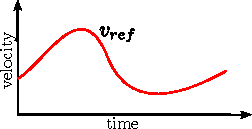
\includegraphics[width=0.6\columnwidth]{images/longitudinal_control.pdf}
    \end{center}
    
    \only<1->{¿Cómo podemos obtener esto?}
    \only<2->{Control PID}
    
\end{frame}


\begin{frame}
    \frametitle{Lateral Control}
    \note{Información extraída de https://youtu.be/pEVsedl2KO4?si=_cwQpRPPUnQ04B3c}
    
    \begin{center}
        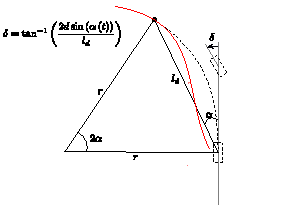
\includegraphics[width=0.6\columnwidth]{images/lateral_control.pdf}
    \end{center}
    
\end{frame}

\begin{frame}
    \frametitle{Control en cascada}
    \note{Información extraída de https://youtu.be/pEVsedl2KO4?si=_cwQpRPPUnQ04B3c}
    
    \begin{center}
        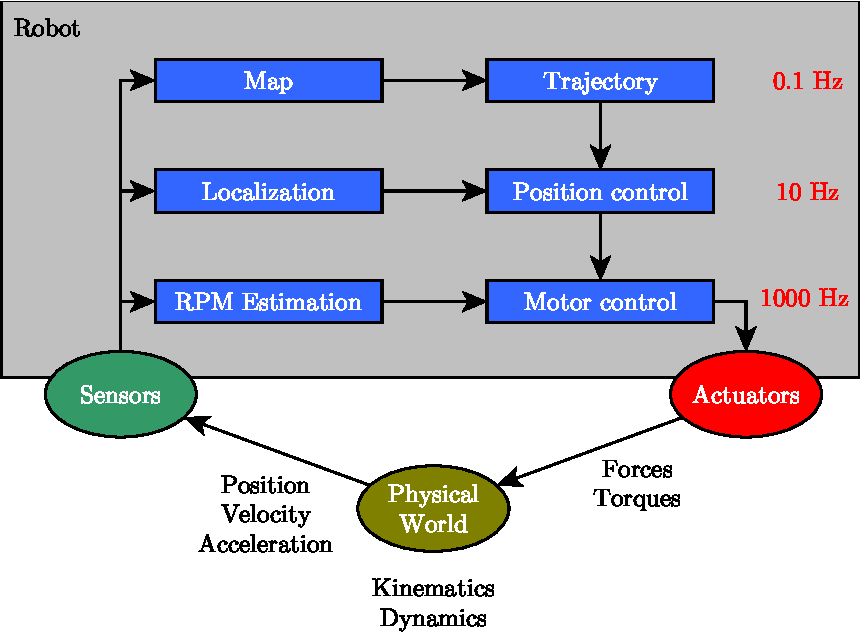
\includegraphics[width=0.7\columnwidth]{./images/control_architecture_phrequency.pdf}
    \end{center}
    
\end{frame}

\begin{frame}
    \frametitle{Objetivos del diseño de control}
    \note{Información extraída de https://youtu.be/pEVsedl2KO4?si=_cwQpRPPUnQ04B3c}
    
    \begin{itemize}
        \item Precisión
        \item Seguridad
        \item Robustez
        \item Tiempo de respuesta
        \item Mantenimiento
        \item y otros objetivos específicos de la aplicación...
    \end{itemize}
    
\end{frame}


\begin{frame}
    \frametitle{Técnicas de control avanzadas}
    \note{Información extraída de https://youtu.be/pEVsedl2KO4?si=_cwQpRPPUnQ04B3c}
    
    \begin{itemize}
        \item Optimal control
        \item Linear Quadratic Regulator (LQR)
        \item Robust control
        \item Adaptive control
        \item Failsafe control
        \item Learning based control
        \item Muchas más técnicas...
    \end{itemize}
    
\end{frame}

\begin{frame}
    \frametitle{Optimal Control}
    \note{Información extraída de https://youtu.be/pEVsedl2KO4?si=_cwQpRPPUnQ04B3c}
    
    \begin{itemize}
        \item Encontrar el controlador que de la mejor performance.
        \item ¿Cómo medir la performance?
        \item ¿Cuál sería una buena medida de performance?
        \begin{itemize}
            \item Minimizar el error?
            \item Minimizar los controles necesarios?
            \item Una combinación de ambas?
        \end{itemize}
    \end{itemize}
    
\end{frame}

\begin{frame}
    \frametitle{Linear Quadratic Regulator (LQR)}
    \note{Información extraída de https://youtu.be/pEVsedl2KO4?si=_cwQpRPPUnQ04B3c}
    
    \begin{itemize}
        \item Sistema \textbf{lineal} de tiempo discreto
        \begin{equation*}
            \state_{k+1} = A \state_{k} + B \controlCommand_{k}
        \end{equation*}
        \item Función de costo \textbf{cuadrática}
        \begin{equation*}
            \jacobian = \sum{\left(\state_{k}^{\top} Q \state_{k} + \controlCommand_{k}^{\top} R \controlCommand_{k}\right)}
        \end{equation*}
        \item \textbf{Objetivo}: Encontrar el control de menor costo.
    \end{itemize}
    
\end{frame}

\begin{frame}
    \frametitle{Control No-lineal}
    \note{Información extraída de https://youtu.be/pEVsedl2KO4?si=_cwQpRPPUnQ04B3c}
    
    \begin{itemize}
        \item ¿Qué si el sistema tiene dinámicas no-lineales?
        \item Resolver un problema de optimización no-lineal es costoso
        \item Linearizar el sistema y resolver como LQR
        \item Resolver el problema de optimización no-lineal para un un horizonte cercano
        \item Resulta en \emph{Model Predictive Controller} (MPC)
    \end{itemize}
    
\end{frame}

\begin{frame}
    \frametitle{Control Adaptativo}
    \note{Información extraída de https://youtu.be/pEVsedl2KO4?si=_cwQpRPPUnQ04B3c}
    
    \begin{itemize}
        \item \textbf{idea:} cambiar la ley de control por la estimarción de parámetros de sistema y actualizarlo en tiempo-real
        \item Adaptar coeficientes basados en meta-observaciones
        \item Lidiar con tiempo variable o incerteza de parámetros
        \item Ejemplo: Decrece en aviones como la masa decrece debido al consumo de combustible 
    \end{itemize}
    
\end{frame}

\begin{frame}
    \frametitle{Control Robusto}
    \note{Información extraída de https://youtu.be/pEVsedl2KO4?si=_cwQpRPPUnQ04B3c}
    
    \begin{itemize}
        \item \textbf{Idea:} Diseño que explícitamente considera la incertidumbre.
        \item Define una cota para la incertidumbre en modelo de parámetros.
        \item La ley de control garantiza estabilidad siempre y cuando la incertidumbre este entre las cotas.
        \item Pero la ley de control es \textbf{estática} a diferencia del control adaptativo.
    \end{itemize}
    
\end{frame}

\begin{frame}
    \frametitle{Control basado en aprendizaje}
    \note{Información extraída de https://youtu.be/pEVsedl2KO4?si=_cwQpRPPUnQ04B3c}
    
    \begin{center}
        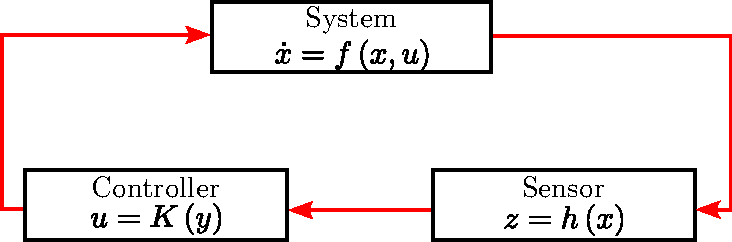
\includegraphics[width=0.7\columnwidth]{./images/learning_based_control.pdf}
    \end{center}
    
\end{frame}

\begin{frame}
    \frametitle{Resumen}
    \note{Información extraída de https://youtu.be/pEVsedl2KO4?si=_cwQpRPPUnQ04B3c}
    
    \begin{itemize}
        \item Motores y controles de bajo nivel
        \item Feedback control
        \item Control PID
        \item Control para seguimiento de caminos
        \item Algunas técnicas de control avanzadas
    \end{itemize}
    
\end{frame}